% Options for packages loaded elsewhere
\PassOptionsToPackage{unicode}{hyperref}
\PassOptionsToPackage{hyphens}{url}
\documentclass[
]{article}
\usepackage{xcolor}
\usepackage[margin=1in]{geometry}
\usepackage{amsmath,amssymb}
\setcounter{secnumdepth}{-\maxdimen} % remove section numbering
\usepackage{iftex}
\ifPDFTeX
  \usepackage[T1]{fontenc}
  \usepackage[utf8]{inputenc}
  \usepackage{textcomp} % provide euro and other symbols
\else % if luatex or xetex
  \usepackage{unicode-math} % this also loads fontspec
  \defaultfontfeatures{Scale=MatchLowercase}
  \defaultfontfeatures[\rmfamily]{Ligatures=TeX,Scale=1}
\fi
\usepackage{lmodern}
\ifPDFTeX\else
  % xetex/luatex font selection
\fi
% Use upquote if available, for straight quotes in verbatim environments
\IfFileExists{upquote.sty}{\usepackage{upquote}}{}
\IfFileExists{microtype.sty}{% use microtype if available
  \usepackage[]{microtype}
  \UseMicrotypeSet[protrusion]{basicmath} % disable protrusion for tt fonts
}{}
\makeatletter
\@ifundefined{KOMAClassName}{% if non-KOMA class
  \IfFileExists{parskip.sty}{%
    \usepackage{parskip}
  }{% else
    \setlength{\parindent}{0pt}
    \setlength{\parskip}{6pt plus 2pt minus 1pt}}
}{% if KOMA class
  \KOMAoptions{parskip=half}}
\makeatother
\usepackage{graphicx}
\makeatletter
\newsavebox\pandoc@box
\newcommand*\pandocbounded[1]{% scales image to fit in text height/width
  \sbox\pandoc@box{#1}%
  \Gscale@div\@tempa{\textheight}{\dimexpr\ht\pandoc@box+\dp\pandoc@box\relax}%
  \Gscale@div\@tempb{\linewidth}{\wd\pandoc@box}%
  \ifdim\@tempb\p@<\@tempa\p@\let\@tempa\@tempb\fi% select the smaller of both
  \ifdim\@tempa\p@<\p@\scalebox{\@tempa}{\usebox\pandoc@box}%
  \else\usebox{\pandoc@box}%
  \fi%
}
% Set default figure placement to htbp
\def\fps@figure{htbp}
\makeatother
\setlength{\emergencystretch}{3em} % prevent overfull lines
\providecommand{\tightlist}{%
  \setlength{\itemsep}{0pt}\setlength{\parskip}{0pt}}
\usepackage{booktabs}
\usepackage{caption}
\usepackage{longtable}
\usepackage{colortbl}
\usepackage{array}
\usepackage{anyfontsize}
\usepackage{multirow}
\usepackage{bookmark}
\IfFileExists{xurl.sty}{\usepackage{xurl}}{} % add URL line breaks if available
\urlstyle{same}
\hypersetup{
  pdftitle={Descriptive Statistics},
  hidelinks,
  pdfcreator={LaTeX via pandoc}}

\title{Descriptive Statistics}
\author{}
\date{\vspace{-2.5em}2026-10-23}

\begin{document}
\maketitle

\begin{verbatim}
## 5th percentile: -1.157863
\end{verbatim}

\begin{verbatim}
## 95th percentile: 0.01086705
\end{verbatim}

\begin{verbatim}
## Observations before trimming: 1223
\end{verbatim}

\begin{verbatim}
## Observations after trimming: 1086
\end{verbatim}

\begin{verbatim}
## Observations removed: 137
\end{verbatim}

\begin{table}[t]
\fontsize{8.0pt}{10.0pt}\selectfont
\begin{tabular*}{\linewidth}{@{\extracolsep{\fill}}l|rrrrrrrr}
\toprule
 & \% of estimates & \% of studies & Mean elasticity & SD elasticity & Min & Max & Mean (SE) & SD (SE) \\ 
\midrule\addlinespace[2.5pt]
{\bfseries Country} &  &  & {} &  &  &  &  &  \\ 
   China & 54.7 & 54.5 & {-0.215} & 0.253 & -1.151 & 0.011 & 0.080 & 0.148 \\ 
   USA & 26.8 & 22.7 & {-0.051} & 0.091 & -0.969 & 0.011 & 0.018 & 0.130 \\ 
   Mexico & 6.2 & 2.3 & {-0.087} & 0.103 & -0.380 & 0.005 & 0.056 & 0.053 \\ 
   India & 4.8 & 6.8 & {-0.054} & 0.058 & -0.228 & 0.008 & 0.018 & 0.012 \\ 
   Germany & 3.6 & 2.3 & {-0.016} & 0.008 & -0.032 & -0.002 & 0.005 & 0.001 \\ 
   Greece & 1.3 & 2.3 & {-0.184} & 0.096 & -0.336 & -0.036 & 0.082 & 0.041 \\ 
   Iran & 1.0 & 2.3 & {-0.168} & 0.127 & -0.351 & -0.061 & 0.073 & 0.050 \\ 
   Canada & 0.6 & 2.3 & {-0.006} & 0.002 & -0.009 & -0.004 & 0.004 & 0.001 \\ 
   Chile & 0.6 & 2.3 & {-0.230} & 0.176 & -0.531 & -0.079 & 0.172 & 0.362 \\ 
   France & 0.5 & 2.3 & {-0.071} & 0.018 & -0.103 & -0.059 & 0.011 & 0.006 \\ 
{\bfseries Development level} &  &  & {} &  &  &  &  &  \\ 
   Non OECD & 60.5 & 63.6 & {-0.201} & 0.245 & -1.151 & 0.011 & 0.075 & 0.142 \\ 
   OECD & 39.5 & 36.4 & {-0.060} & 0.096 & -0.969 & 0.011 & 0.028 & 0.117 \\ 
{\bfseries Localisation (urban / rural)} &  &  & {} &  &  &  &  &  \\ 
   Mixed & 49.1 & 54.5 & {-0.198} & 0.251 & -1.151 & 0.011 & 0.086 & 0.159 \\ 
   Urban & 31.4 & 29.5 & {-0.122} & 0.163 & -1.107 & 0.009 & 0.039 & 0.125 \\ 
   NA & 12.1 & 9.1 & {-0.025} & 0.035 & -0.177 & 0.006 & 0.006 & 0.013 \\ 
   Rural & 7.5 & 6.8 & {-0.092} & 0.168 & -1.024 & 0.000 & 0.035 & 0.061 \\ 
{\bfseries Indoor or outdoor workers} &  &  & {} &  &  &  &  &  \\ 
   Indoor & 42.3 & 40.9 & {-0.139} & 0.190 & -1.151 & 0.009 & 0.047 & 0.126 \\ 
   Outdoor & 41.6 & 25.1 & {-0.105} & 0.151 & -1.046 & 0.011 & 0.052 & 0.138 \\ 
   Mixed & 14.6 & 31.8 & {-0.250} & 0.322 & -1.125 & 0.006 & 0.090 & 0.138 \\ 
   NA & 1.5 & 2.1 & {-0.428} & 0.335 & -1.107 & -0.037 & 0.147 & 0.163 \\ 
{\bfseries Mean Age} & 30.0 & 32.7 & {} &  &  &  &  &  \\ 
{\bfseries Female} & 2.6 & 3.1 & {} &  &  &  &  &  \\ 
{\bfseries Sector} &  &  & {} &  &  &  &  &  \\ 
   Service & 34.4 & 27.3 & {-0.158} & 0.198 & -1.151 & 0.011 & 0.072 & 0.177 \\ 
   Sport & 30.3 & 20.5 & {-0.083} & 0.110 & -0.408 & 0.011 & 0.021 & 0.031 \\ 
   Industry & 23.3 & 34.1 & {-0.237} & 0.300 & -1.125 & 0.009 & 0.089 & 0.139 \\ 
   Agriculture & 7.5 & 6.8 & {-0.092} & 0.168 & -1.024 & 0.000 & 0.035 & 0.061 \\ 
   NA & 3.5 & 6.8 & {-0.034} & 0.132 & -0.814 & 0.001 & 0.011 & 0.051 \\ 
   Mixed & 1.0 & 4.5 & {-0.241} & 0.139 & -0.531 & -0.079 & 0.122 & 0.263 \\ 
{\bfseries Task type} &  &  & {} &  &  &  &  &  \\ 
   Physical & 55.2 & 39.4 & {-0.136} & 0.188 & -1.151 & 0.011 & 0.056 & 0.128 \\ 
   Cognitive & 30.8 & 31.1 & {-0.073} & 0.114 & -0.969 & 0.008 & 0.028 & 0.116 \\ 
   Mixed & 14.0 & 29.5 & {-0.342} & 0.320 & -1.125 & 0.002 & 0.129 & 0.171 \\ 
{\bfseries Productivity measures} &  &  & {} &  &  &  &  &  \\ 
   Piece rate & 25.0 & 13.6 & {-0.151} & 0.178 & -1.107 & 0.011 & 0.072 & 0.150 \\ 
   Output/worker & 23.0 & 32.8 & {-0.262} & 0.321 & -1.151 & 0.009 & 0.096 & 0.143 \\ 
   Physical performance & 21.1 & 15.9 & {-0.111} & 0.119 & -0.388 & 0.011 & 0.030 & 0.036 \\ 
   Cognitive performance & 10.2 & 9.1 & {-0.013} & 0.041 & -0.345 & 0.006 & -0.003 & 0.019 \\ 
   Time spent output & 7.8 & 4.5 & {-0.120} & 0.121 & -0.548 & 0.005 & 0.045 & 0.052 \\ 
   Time spent & 4.8 & 3.2 & {-0.036} & 0.054 & -0.408 & -0.005 & 0.006 & 0.004 \\ 
   Output & 4.5 & 4.5 & {-0.090} & 0.083 & -0.336 & -0.008 & 0.031 & 0.046 \\ 
   Financial index & 2.3 & 4.5 & {-0.212} & 0.233 & -0.969 & 0.005 & 0.112 & 0.398 \\ 
   Wage & 0.7 & 6.8 & {-0.285} & 0.403 & -1.046 & -0.059 & 0.259 & 0.457 \\ 
   NA & 0.3 & 2.6 & {-0.126} & 0.226 & -0.386 & 0.008 & 0.076 & 0.102 \\ 
   Other & 0.2 & 2.3 & {-0.016} & 0.004 & -0.019 & -0.013 & 0.015 & 0.001 \\ 
{\bfseries Aggregation level} &  &  & {} &  &  &  &  &  \\ 
   Worker & 71.7 & 52.5 & {-0.105} & 0.145 & -1.107 & 0.011 & 0.039 & 0.099 \\ 
   Other & 15.8 & 20.2 & {-0.085} & 0.155 & -1.024 & 0.009 & 0.047 & 0.179 \\ 
   Firm & 12.4 & 27.3 & {-0.456} & 0.315 & -1.151 & 0.002 & 0.179 & 0.180 \\ 
{\bfseries Pollution measures} &  &  & {} &  &  &  &  &  \\ 
   PM2.5 & 30.3 & 47.9 & {-0.163} & 0.243 & -1.151 & 0.011 & 0.064 & 0.175 \\ 
   O3 & 26.1 & 14.6 & {-0.146} & 0.168 & -1.024 & 0.010 & 0.074 & 0.150 \\ 
   AQI & 13.1 & 10.9 & {-0.150} & 0.129 & -0.459 & 0.003 & 0.032 & 0.046 \\ 
   NO2 & 6.9 & 3.9 & {-0.042} & 0.069 & -0.347 & 0.001 & 0.020 & 0.029 \\ 
   PM10 & 6.4 & 6.2 & {-0.098} & 0.121 & -0.429 & 0.003 & 0.052 & 0.069 \\ 
   CO & 5.1 & 2.9 & {-0.040} & 0.074 & -0.276 & 0.011 & 0.009 & 0.020 \\ 
   API & 4.6 & 4.5 & {-0.153} & 0.269 & -1.107 & -0.003 & 0.054 & 0.112 \\ 
   SO2 & 4.2 & 2.3 & {-0.124} & 0.277 & -0.999 & 0.009 & 0.040 & 0.094 \\ 
   PM1 & 2.7 & 2.3 & {-0.548} & 0.369 & -1.125 & -0.011 & 0.252 & 0.146 \\ 
   NOx & 0.5 & 2.3 & {-0.071} & 0.018 & -0.103 & -0.059 & 0.011 & 0.006 \\ 
   Emission of industrial waste gases & 0.2 & 2.3 & {-0.016} & 0.004 & -0.019 & -0.013 & 0.015 & 0.001 \\ 
{\bfseries Pollution method measurement} &  &  & {} &  &  &  &  &  \\ 
   Fixed station & 89.2 & 70.5 & {-0.101} & 0.138 & -1.107 & 0.011 & 0.040 & 0.112 \\ 
   Satellite & 10.6 & 27.3 & {-0.519} & 0.327 & -1.151 & 0.002 & 0.205 & 0.208 \\ 
   NA & 0.2 & 2.3 & {-0.016} & 0.004 & -0.019 & -0.013 & 0.015 & 0.001 \\ 
{\bfseries Data structure} &  &  & {} &  &  &  &  &  \\ 
   Panel & 95.0 & 93.2 & {-0.150} & 0.214 & -1.151 & 0.011 & 0.058 & 0.123 \\ 
   Cross-sectional & 3.5 & 4.2 & {-0.049} & 0.062 & -0.408 & -0.016 & 0.007 & 0.004 \\ 
   Time serie & 1.5 & 2.5 & {-0.066} & 0.241 & -0.969 & 0.005 & 0.127 & 0.495 \\ 
{\bfseries Frequency} &  &  & {} &  &  &  &  &  \\ 
   Other & 46.4 & 38.5 & {-0.093} & 0.136 & -1.107 & 0.011 & 0.026 & 0.052 \\ 
   Daily & 40.9 & 25.1 & {-0.105} & 0.139 & -0.969 & 0.011 & 0.052 & 0.151 \\ 
   Yearly & 12.7 & 36.4 & {-0.466} & 0.324 & -1.151 & 0.002 & 0.185 & 0.195 \\ 
{\bfseries Estimation method} &  &  & {} &  &  &  &  &  \\ 
   Semi elasticity & 43.2 & 38.3 & {-0.180} & 0.228 & -1.151 & 0.011 & 0.080 & 0.142 \\ 
   Marginal effect & 32.0 & 31.0 & {-0.061} & 0.118 & -1.046 & 0.011 & 0.028 & 0.141 \\ 
   Elasticity & 16.6 & 26.4 & {-0.207} & 0.281 & -1.125 & 0.002 & 0.060 & 0.120 \\ 
   Level-log & 8.3 & 4.4 & {-0.168} & 0.132 & -0.388 & 0.007 & 0.034 & 0.041 \\ 
{\bfseries Identification strategy} &  &  & {} &  &  &  &  &  \\ 
   OLS & 54.5 & 55.5 & {-0.071} & 0.122 & -1.024 & 0.011 & 0.021 & 0.095 \\ 
   IV & 42.4 & 41.4 & {-0.220} & 0.238 & -1.151 & 0.009 & 0.095 & 0.159 \\ 
         Thermal inversion & 70.0 & 59.7 & {-0.239} & 0.242 & -1.151 & 0.009 & 0.095 & 0.165 \\ 
         Other instrument & 30.0 & 40.3 & {-0.176} & 0.224 & -1.151 & 0.005 & 0.093 & 0.144 \\ 
   Other & 3.1 & 3.1 & {-0.432} & 0.395 & -1.125 & 0.001 & 0.179 & 0.167 \\ 
{\bfseries Fixed effects} &  &  & {} &  &  &  &  &  \\ 
   Time FE & 95.2 & 91.3 & {-0.149} & 0.215 & -1.151 & 0.011 & 0.059 & 0.138 \\ 
   Worker FE & 58.7 & 38.5 & {-0.105} & 0.150 & -1.107 & 0.011 & 0.048 & 0.121 \\ 
   Firm FE & 27.7 & 41.8 & {-0.251} & 0.294 & -1.151 & 0.005 & 0.094 & 0.134 \\ 
   Localisation FE & 12.2 & 20.7 & {-0.210} & 0.279 & -1.151 & 0.003 & 0.077 & 0.156 \\ 
   No fixed effects & 1.7 & 2.9 & {-0.057} & 0.086 & -0.287 & 0.000 & 0.018 & 0.023 \\ 
{\bfseries Weather controls} &  &  & {} &  &  &  &  &  \\ 
   Weather controls & 82.5 & 78.3 & {-0.144} & 0.204 & -1.151 & 0.011 & 0.060 & 0.139 \\ 
         Temperature & 81.6 & 72.5 & {-0.144} & 0.203 & -1.151 & 0.011 & 0.059 & 0.132 \\ 
         Wind speed & 74.1 & 64.1 & {-0.151} & 0.210 & -1.151 & 0.011 & 0.063 & 0.146 \\ 
         Humidity & 52.4 & 52.0 & {-0.177} & 0.234 & -1.151 & 0.011 & 0.074 & 0.144 \\ 
         Other & 85.5 & 91.8 & {-0.172} & 0.230 & -1.151 & 0.011 & 0.069 & 0.159 \\ 
   No weather controls & 17.5 & 21.7 & {-0.151} & 0.244 & -1.125 & 0.009 & 0.043 & 0.113 \\ 
{\bfseries Other pollutant controls} &  &  & {} &  &  &  &  &  \\ 
   Multiple pollutants & 30.1 & 18.7 & {-0.060} & 0.117 & -0.969 & 0.011 & 0.031 & 0.125 \\ 
   No multiple pollutants & 69.9 & 81.3 & {-0.182} & 0.232 & -1.151 & 0.009 & 0.068 & 0.137 \\ 
{\bfseries Other controls} &  &  & {} &  &  &  &  &  \\ 
   Worker characteristics & 3.9 & 4.5 & {-0.030} & 0.055 & -0.273 & -0.002 & 0.012 & 0.026 \\ 
   Attendance bias & 79.7 & 52.2 & {-0.096} & 0.136 & -1.107 & 0.011 & 0.038 & 0.094 \\ 
   Traffic controls & 0.4 & 0.3 & {-0.012} & 0.011 & -0.022 & -0.003 & 0.007 & 0.002 \\ 
   Demand controls & 0.4 & 0.3 & {-0.018} & 0.003 & -0.021 & -0.014 & 0.008 & 0.002 \\ 
   Wage / shirking controls & 0.0 & 0.0 & {} &  &  &  &  &  \\ 
\bottomrule
\end{tabular*}
\begin{minipage}{\linewidth}
\vspace{.05em}
Note: under IV, the shares are computed among IV estimates only.\\
\end{minipage}
\end{table}

\pandocbounded{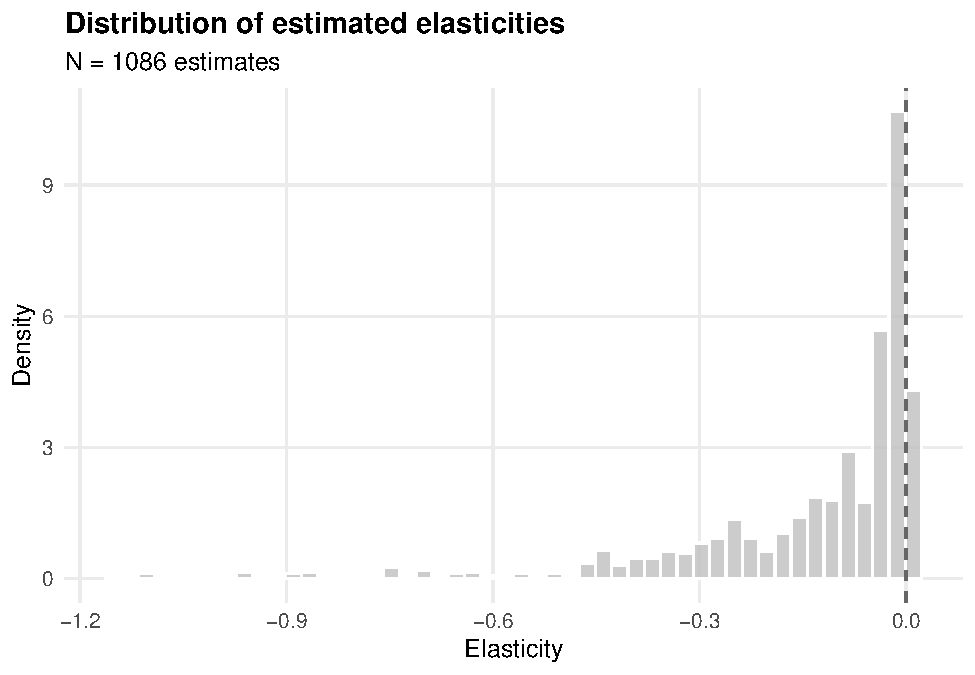
\includegraphics[keepaspectratio]{Descriptive_statistics_files/Descriptive_statistics_files/figure-latex/unnamed-chunk-3-1.pdf}}
\pandocbounded{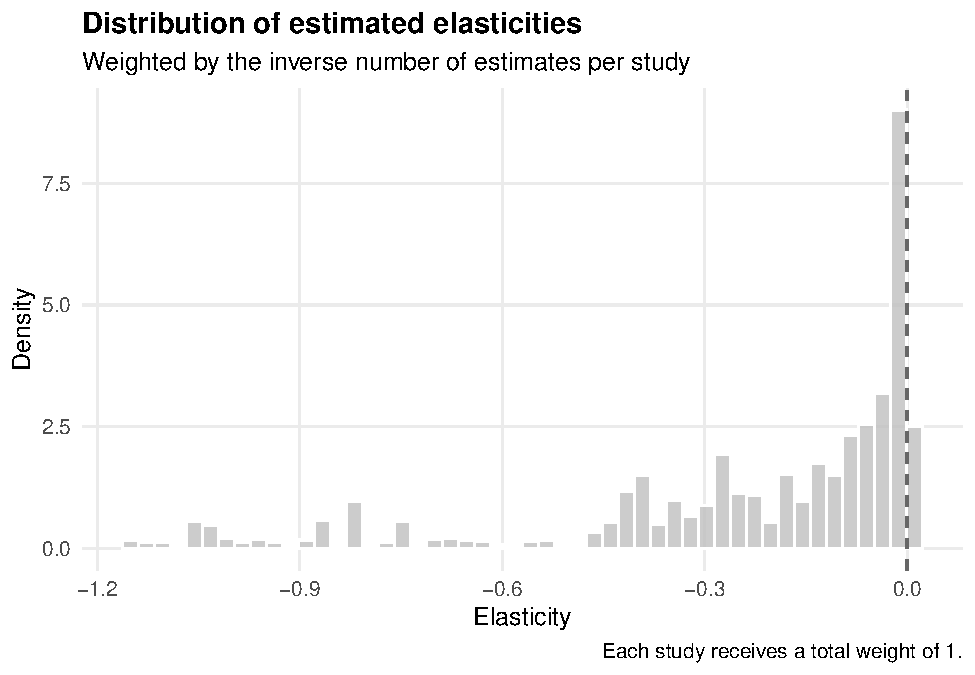
\includegraphics[keepaspectratio]{Descriptive_statistics_files/Descriptive_statistics_files/figure-latex/unnamed-chunk-3-2.pdf}}

\pandocbounded{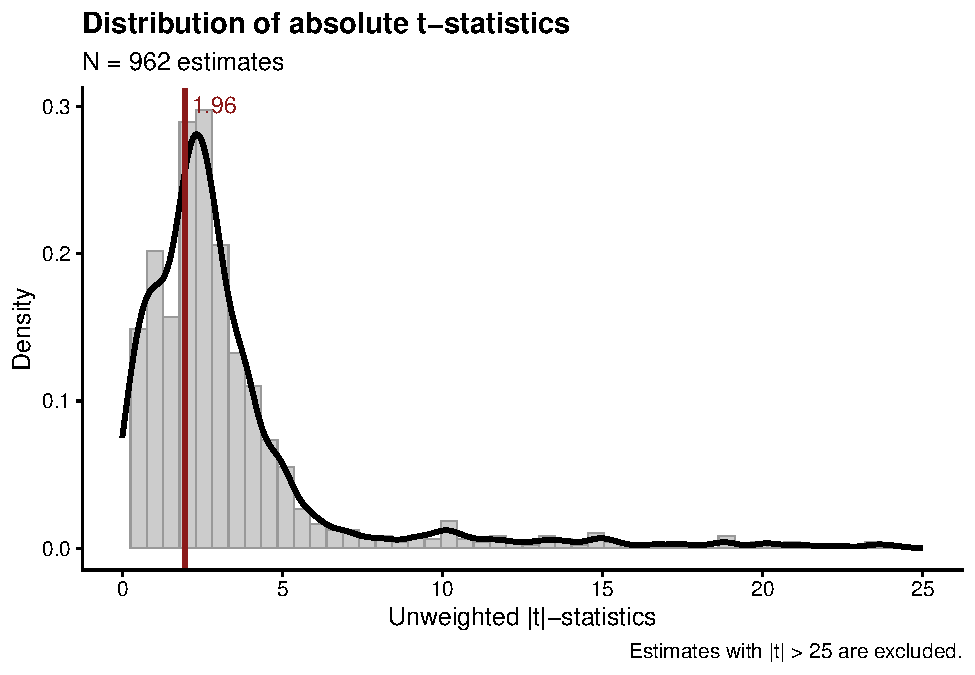
\includegraphics[keepaspectratio]{Descriptive_statistics_files/Descriptive_statistics_files/figure-latex/unnamed-chunk-4-1.pdf}}
\pandocbounded{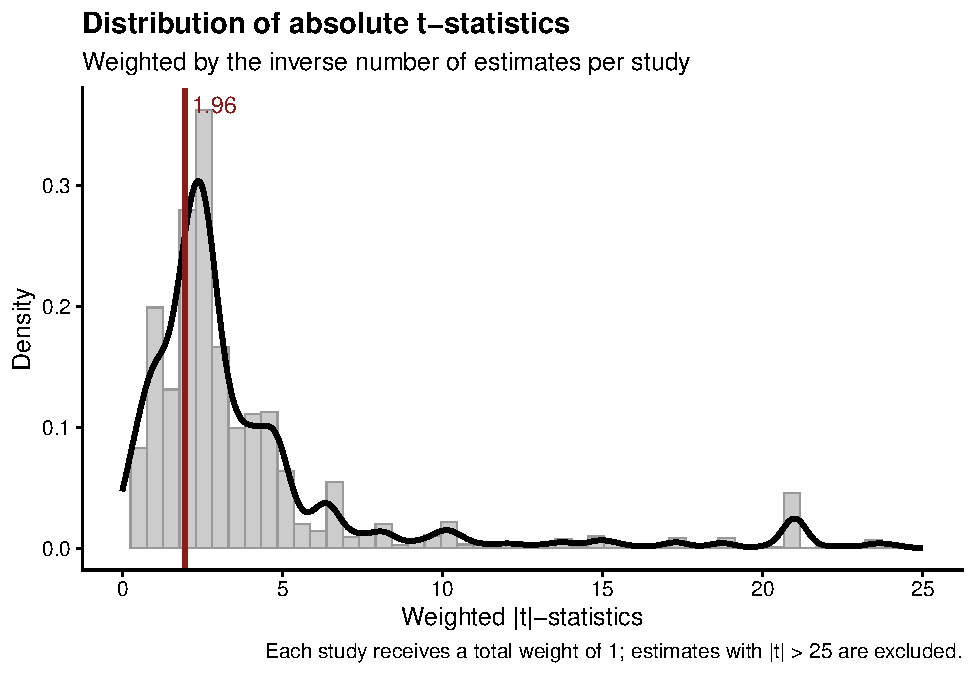
\includegraphics[keepaspectratio]{Descriptive_statistics_files/Descriptive_statistics_files/figure-latex/unnamed-chunk-4-2.pdf}}

\pandocbounded{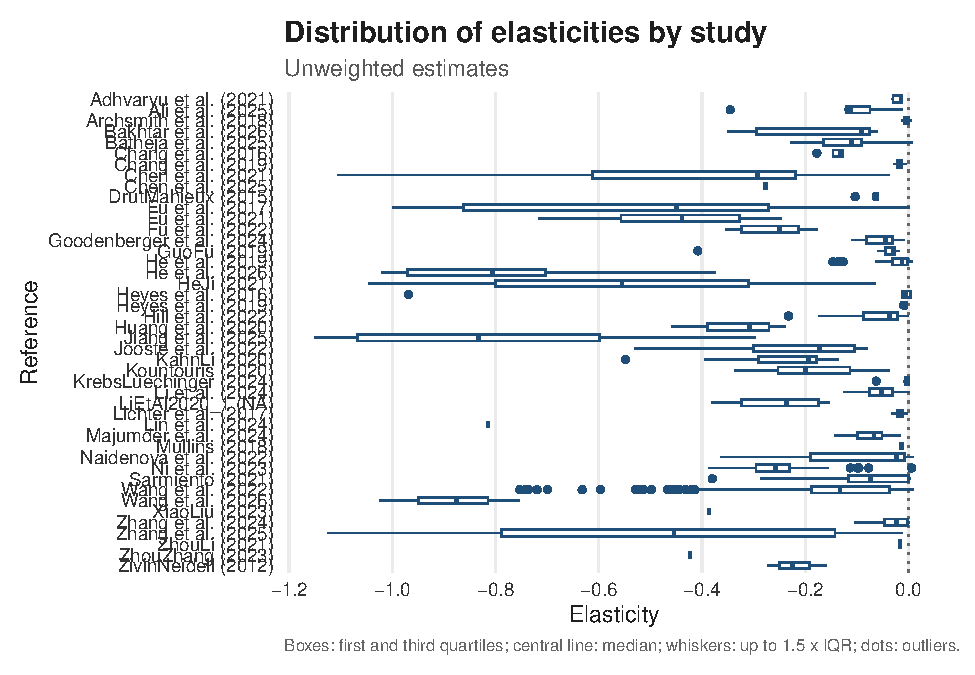
\includegraphics[keepaspectratio]{Descriptive_statistics_files/Descriptive_statistics_files/figure-latex/unnamed-chunk-5-1.pdf}}
\pandocbounded{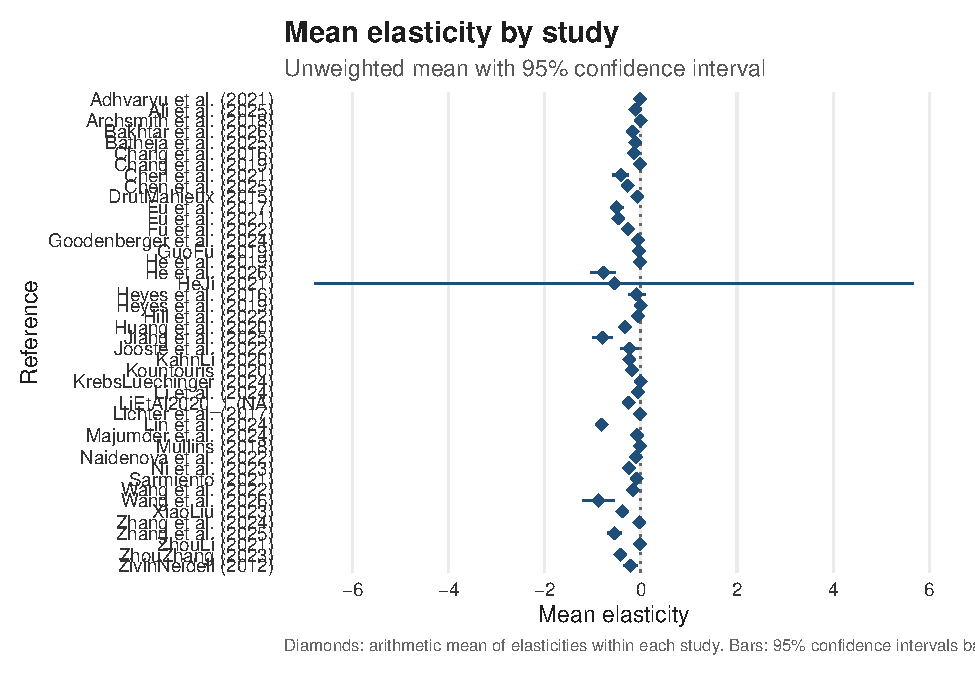
\includegraphics[keepaspectratio]{Descriptive_statistics_files/Descriptive_statistics_files/figure-latex/unnamed-chunk-5-2.pdf}}

\pandocbounded{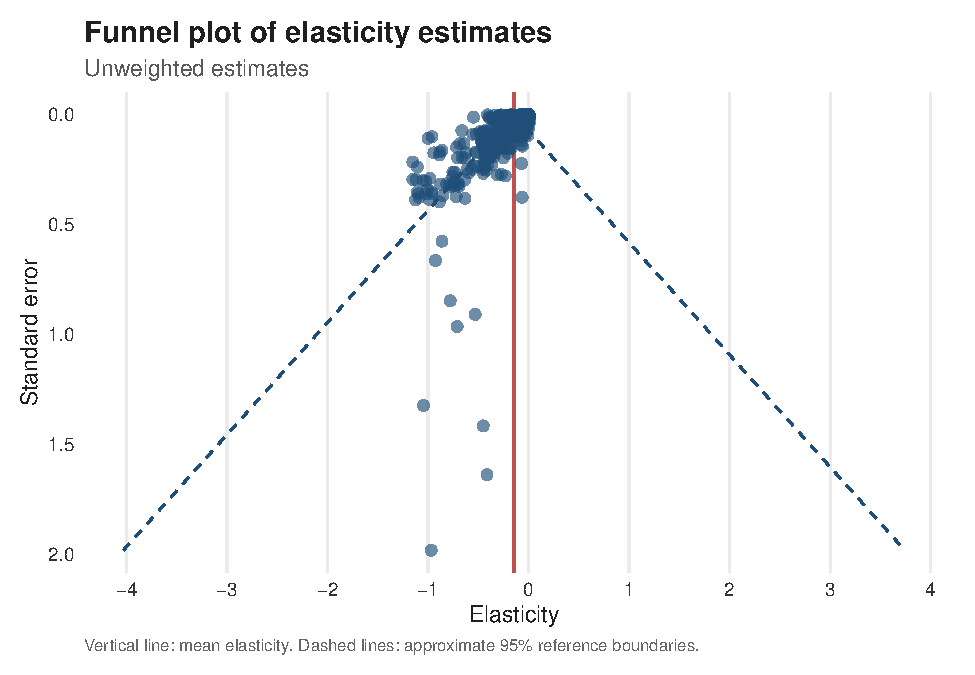
\includegraphics[keepaspectratio]{Descriptive_statistics_files/Descriptive_statistics_files/figure-latex/unnamed-chunk-6-1.pdf}}

\end{document}
